
%\usepackage{enumitem}
\chapter{Análise de desempenho do Blockchain}
\label{chapter_desempenho}


      O Blockchain é amplamente reconhecido hoje como uma tecnologia disruptiva com o potencial de transformar diversos setores. Sua capacidade de oferecer um registro distribuído seguro e imutável abriu caminho para inovações em finanças, cadeia de suprimentos, saúde e muitos outros campos. À medida que diversas plataformas e projetos adotam essa tecnologia, torna-se imperativo avaliar seu desempenho em diversos contextos. Neste contexto, iremos explorar as diferentes dimensões do desempenho do blockchain, com ênfase especial em uma métrica-chave e uma análise aprofundada

\section{Métrica do Desempenho}

    A medida do desempenho do Blockchain e a metrica para a velocidade das transações são conceitos que evoluíram ao longo do tempo à medida que a technologia blockchain se desenvolveu. Uma das metricas mais frequentemente consideradas é a "velocidade de transações" ou "transaçoes por segundos(TPS)", que mede quantas transões a rede blockchain pode processar em um determinado periodo. 

\subsection{Mediçaõ do desempenho do Blockchain}
    A medição do desempenho do Blockchain começou a ganhar destaque logo após o lançamento do Bitcoin em 2009.
    Como foi especificado no meu desenvolvimento , o Bitcoin do Satochi foi a primeira implementação pratica da tecnologia blockchain, e a medida que a rede crescia, surgiram preocupações sobre sua capacidade de lidar com um grande número de transações .Isso que levou a discussões sobre a escalabilidade e eficiência da rede , inaugurando uma era de medição de desempenho mais sistemática. Uma lista representativa de pesquisas existentes, mostrada na tabela abaixo , identificando a necessidade pesquisas sistematica sobre a avaliação do desempenho do blockchain.
\begin{table}[H]
%\centering
\renewcommand{\arraystretch}{2} % Ajustez le facteur selon vos besoins
\begin{tabular}{|>{\bfseries}l|c|p{7cm}|}
\hline
\textbf{Year} & \textbf{Survey} & \textbf{Research Scope} \\
\hline
2018 & Kim et al.\cite{kim2018survey} & Escalability Solution\\
\hline
2019 & Rouhani and Deters\cite{rouhani2019security} & security, performance, and applications of smart contract\\
\hline
2019 & Zheng et al.\cite{zheng2019survey}  & challenges of performance and security\\
\hline
2019 & Wang et al. \cite{alpak2021benchmarking} & benchmarking tools and performance optimization methods\\
\hline
2020 & Zhou et al. \cite{zhou2020solutions}  & scaling solutions to blockchain\\
\hline
2020 & Yu et al. \cite{xie2019survey}  & sharding for blockchain scalability \\
\hline
\end{tabular}
\caption{Escopo de pesquisas relacionados aos desempenhos existentes.}
\label{tab:Escopo de pesquisas relacionados aos desempenhos existentes}
\end{table}

\subsection{Metricas para velocidade das transaçoes}

    A métrica para a velocidade das transações, conhecida como "transações por segundo" (TPS), tornou-se relevante à medida que o Bitcoin e outras criptomoedas ganhavam popularidade. A TPS é uma métrica simples que representa o número de transações que uma rede blockchain pode processar em um segundo. Ela se tornou importante devido às diversas razões tais como:

    \begin{itemize}
    \item Concorencia com Sistemas Financeiros Tradicionais : À medida que as criptomoedas começaram a competir com sistemas financeiros tradicionais, a capacidade de processar transações rapidamente se tornou um ponto crítico de avaliação. Os sistemas de pagamento tradicionais, como cartões de crédito, processam milhares de transações por segundo, e o blockchain precisava demonstrar sua capacidade de competir nesse aspecto.
    
    \item Congestionamento da Rede : Com o aumento do uso, o Bitcoin enfrentou congestionamentos na rede que levaram a atrasos nas transações e ao aumento das taxas de transação. A métrica TPS se tornou uma maneira clara de avaliar a capacidade da rede de lidar com a demanda. 
    \item Melhorias da tednologia : A busca por aumentar a TPS levou ao desenvolvimento de novas tecnologias e algoritmos de consenso, como o Segregated Witness (SegWit) no Bitcoin e o Ethereum 2.0. Essas melhorias foram impulsionadas pela necessidade de aumentar o desempenho.
    
    \end{itemize}
    Portanto, a métrica TPS surgiu organicamente da necessidade de avaliar a capacidade do blockchain de processar transações de forma eficiente e competir com sistemas financeiros existentes. Desde então, ela se tornou uma métrica padrão para medir o desempenho de redes blockchain e continua a evoluir à medida que novas soluções são desenvolvidas para melhorar a escalabilidade e a eficiência das redes blockchain.

    \section{Análise de desempenho Blockchain baseada em Evidencias}

    A "Analíse de desempenho Blockchain Baseada em Evidências " representa uma abordagem essential na avaliação critica da tecnologia blockchain .À medida que os bockchains continuam a se difundir em diversos setores , a necessidade de uma avaliação fundamentada em dados torna-se cada vez mais premente. Esta analise empírica não apenas permite a comprensão aprofundada do funcionamento de sistema blockchain, mas também ajuda a tomar decisões informadas sobre a sua implementação.Neste texto, exploraremos a importância e os métodos dessa análise baseada em evidências, destacando como ela pode moldar o futuro dessas tecnologias disruptivas. 
    As abordagens de avaliação revistas podem ser categorizadas em dois grupos principais: avaliação empírica e modelagem analítica, conforme demonstrado na figura  \ref{Blockchain-Evaluation}.

        \begin{figure}[H]
            \centering
            \frame{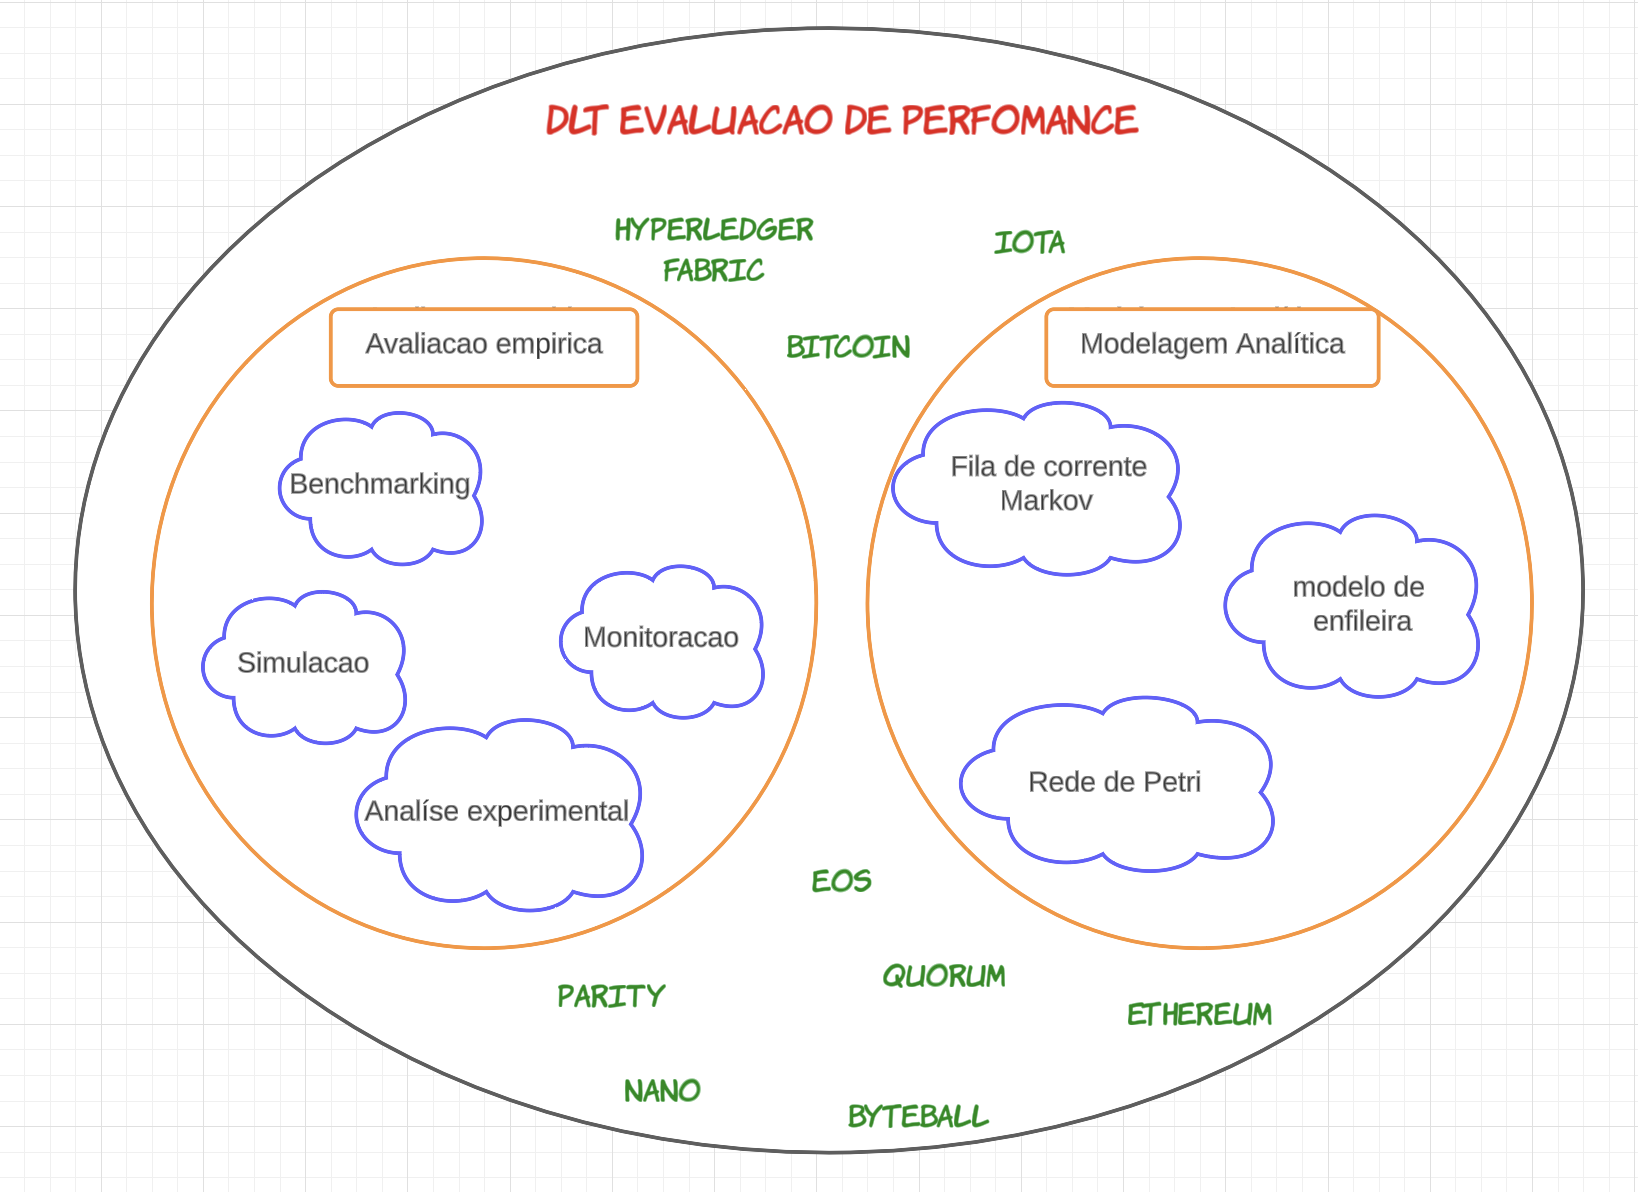
\includegraphics[width=15cm]{4-Analise-de-desempenho-do-Blockchain/figure/abordagem.png}}
            \caption{Cenário de abordagens de avaliação de desempenho DLT e livros-razão avaliados. \cite{9129732}, .}
            \label{Blockchain-Evaluation}
        \end{figure}

    
    \subsection{\ Instrumentos de Benchmarking Blockchain}

     \textbf{O Benchmarking} é uma prática essencial na avaliação do desempenho do blockchain. Essas ferramentas são projetadas para medir e comparar o desempenho de diferentes sistemas blockchain em relação a métricas específicas.
     O benchmarking de desempenho tem sido extensivamente pesquisado e documentado em relação a sistemas de nuvem, como Hadoop, MapReduce e Spark, bem como em sistemas de banco de dados, abrangendo sistemas relacionais e NoSQL.\cite{9129732}
     O surgimento constante de sistemas blockchain, que buscam aprimorar o desempenho do Ledger Distribuído (DTL), torna-se imperativo desenvolver uma solução capaz de comparar as diversas plataformas de maneira significativa.

     Até junho de 2020  exitem três Benchmarks Populares de Blockchain dedicados à avaliação de sistemas de blockchain, conforme listado na Tabela  \ref{Blockchain-Comparison}.


\begin{figure} [H]
\centering
\frame{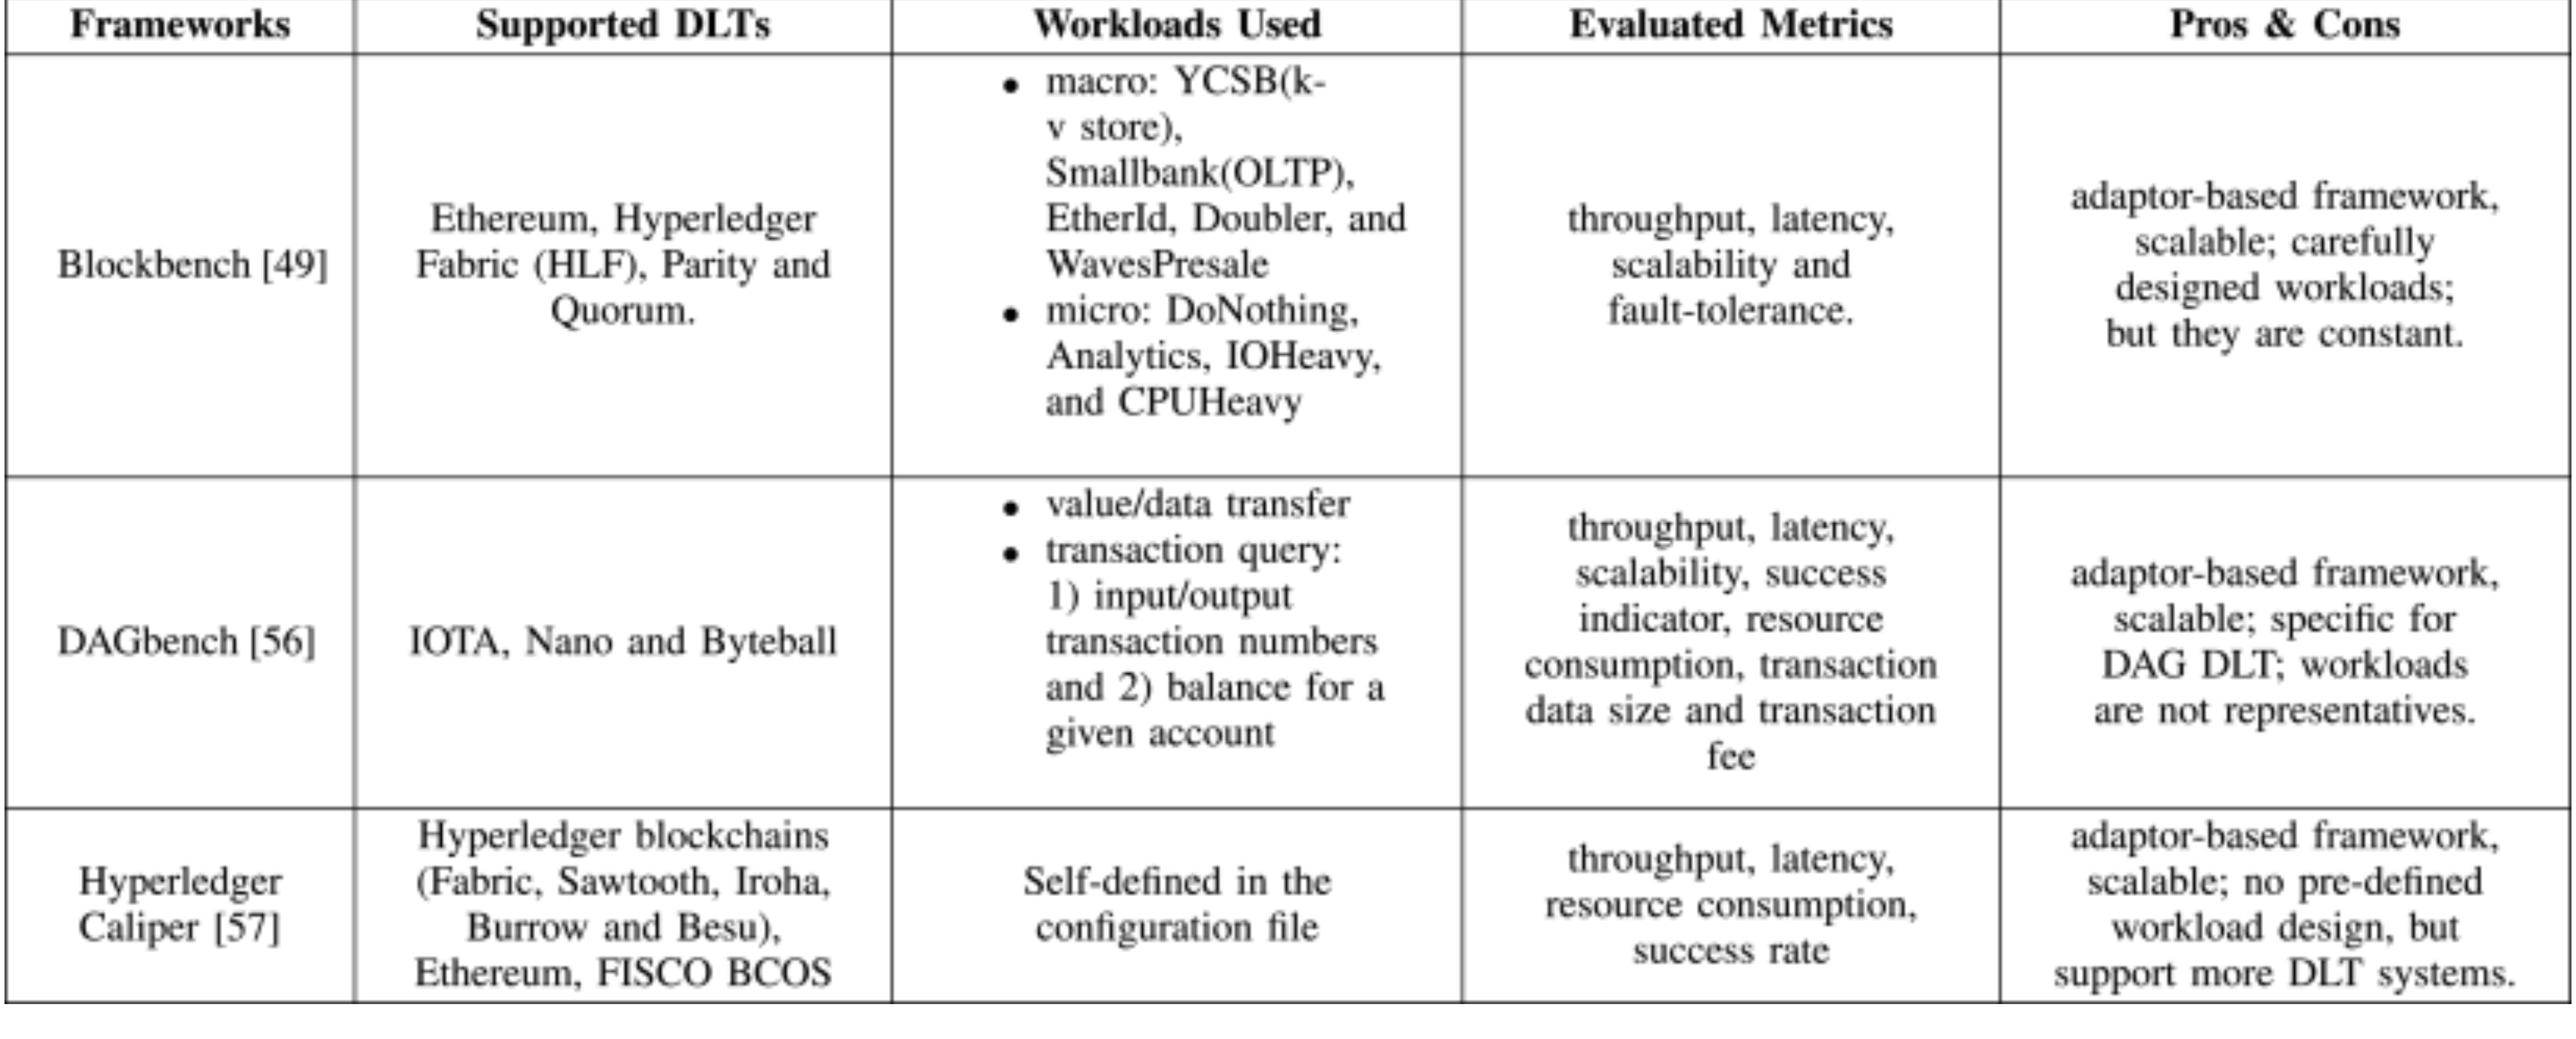
\includegraphics[width=15cm]{4-Analise-de-desempenho-do-Blockchain/figure/comparacao de tres cenchmarks.png}}
\caption{Comparação de Três Benchmarks PoPulares de Blockchain, \cite{9129732}, .}
\label{Blockchain-Comparison}
\end{figure}
\textbf{O BlockBench} é uma ferramenta de de benchmarking amplamente utilizada para avaliar o desempenho de sistemas blockchain . Ela oferece um ambiente de simulação que permite aos pesquisadores e desenvolvedores testar e comparar o desempenho de diferentes blockchains sob várias condições controladas. Atualemente ele suporta medição de em quatro grandes plataformas privadas de blockchains , a saber , Etherium , Parity,HLF e Quorum.
No design do BlockBench, formam identificadas quatro camadas de abstração que desempenham papéis essenciais no funcionamento de sistemas blockchain. Essas camadas são organizadas em uma hieraquia que vai desde o nível mais baixo até o nivel maos alto. Figure \ref{BlockBench-Layers}

\begin{itemize}[label=$\blacksquare$]
\item \textbf{Camada de Consenso:} A camada mais fundamental é a de consenso. Aqui, as regras de acordo são estabelecidas e implementadas para garantir que todos os participantes da rede cheguem a um consenso sobre o conteúdo que será adicionado a um bloco e, subsequentemente, ao blockchain. É nessa camada que são definidos os algoritmos de consenso que garantem a integridade e a validade das transações.

\item \textbf{Camada de Modelo de Dados:} A camada de modelo de dados é responsável por definir a estrutura, o conteúdo e as operações que podem ser realizadas nos dados armazenados no blockchain. Essa camada desempenha um papel crucial na definição das informações que podem ser registradas no blockchain e na forma como esses dados são organizados.

\item \textbf{Camada de Mecanismo de Execução:} A terceira camada, o mecanismo de execução, abrange o ambiente de tempo de execução, onde ocorre a execução de códigos e contratos inteligentes. Nela, estão presentes recursos essenciais, como a Máquina Virtual Ethereum (EVM) e tecnologias como Docker, que oferecem suporte às operações de execução nos blockchains. Essa camada permite que os contratos inteligentes sejam executados e que as ações programadas sejam processadas com eficiência.

\item \textbf{Camada de Aplicativos:} Por fim, a camada de aplicativos é o nível mais alto da hierarquia. Nessa camada, encontram-se diversos tipos de aplicativos blockchain, incluindo contratos inteligentes e Decentralized Applications (DApps). Aqui é onde a funcionalidade real é entregue aos usuários e aplicativos, abrangendo uma ampla gama de casos de uso, desde finanças descentralizadas até cadeias de suprimentos transparentes.

\end{itemize}

        \begin{figure}[H]
            \centering
            \frame{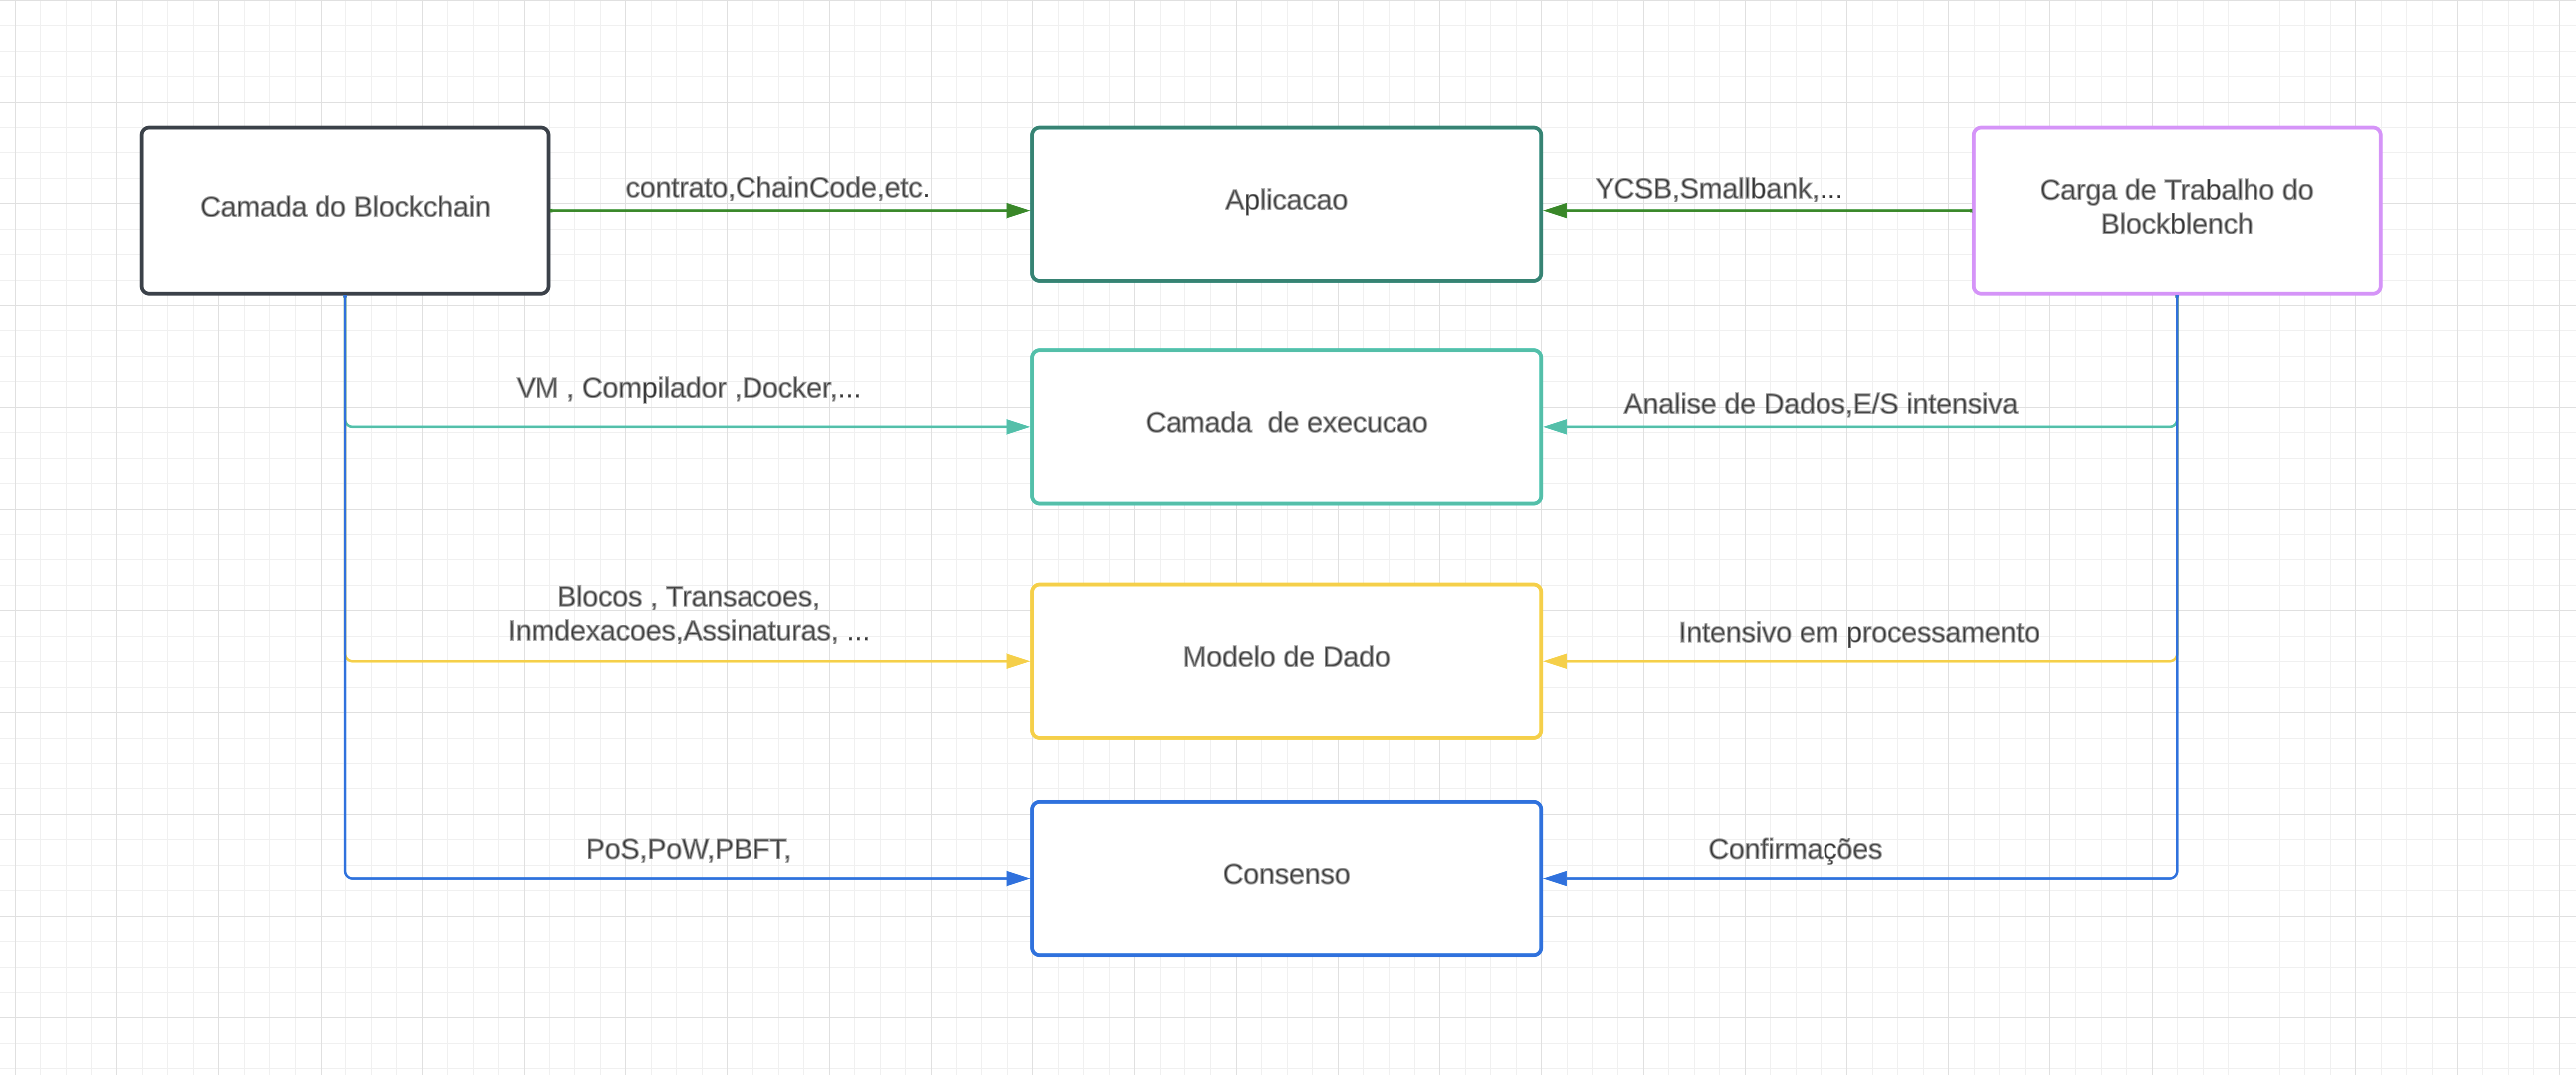
\includegraphics[width=15cm]{4-Analise-de-desempenho-do-Blockchain/figure/abstracao_de_camad.png}}
            \caption{Abstraction layers in blockchain, and the corresponding workloads in BLOCKBENCH. \cite{blockbench}, .}
            \label{BlockBench-Layers}
        \end{figure}

    \subsection{Supervisionamento do desempenho do Blockchain}

    A prática de benchmarking em blockchains geralmente demanda um ambiente padronizado e uma carga de trabalho bem documentada como entradas. No entanto, quando se trata de sistemas públicos de blockchain, enfrentamos desafios adicionais devido à impossibilidade de controlar totalmente a carga de trabalho real e os participantes do consenso. Isso torna o benchmarking uma tarefa mais complexa. No contexto da avaliação de blockchains públicos, duas abordagens têm se destacado.

    A primeira abordagem envolve a criação de uma versão privada da rede de teste correspondente e o subsequente uso de benchmarks já existentes, conforme mencionados anteriormente, para avaliar o desempenho do blockchain sob cargas de trabalho artificialmente projetadas. Essa estratégia pode requerer o desenvolvimento de um novo adaptador para cargas de trabalho ou a configuração de uma rede blockchain privada específica. No entanto, é importante notar que essa abordagem deve lidar com o desafio da escalabilidade do blockchain. A versão privada testada do blockchain pode não refletir completamente os problemas de escalabilidade que podem surgir quando a implementação acontece em um ambiente público. Portanto, os resultados obtidos nesse ambiente controlado podem apresentar valores de métricas de desempenho mais otimistas em comparação com a rede pública real.

    A segunda abordagem consiste em monitorar e avaliar o desempenho do sistema público em tempo real, sob cargas de trabalho realistas.Zheng et al. \cite{zhou2020solutions} propuseram uma estrutura abrangente de monitoramento de desempenho em tempo real que utiliza uma abordagem baseada em registros. Essa abordagem apresenta vantagens, como menor sobrecarga, detalhes mais abrangentes e melhor escalabilidade, em comparação com a solução que faz uso de chamadas de procedimento remoto (RPC) como contraparte. Isso permite uma avaliação mais precisa do desempenho do sistema em um ambiente de produção, onde a carga de trabalho reflete situações reais de uso.\cite{9129732}


        \begin{figure}[H]
            \centering
            \frame{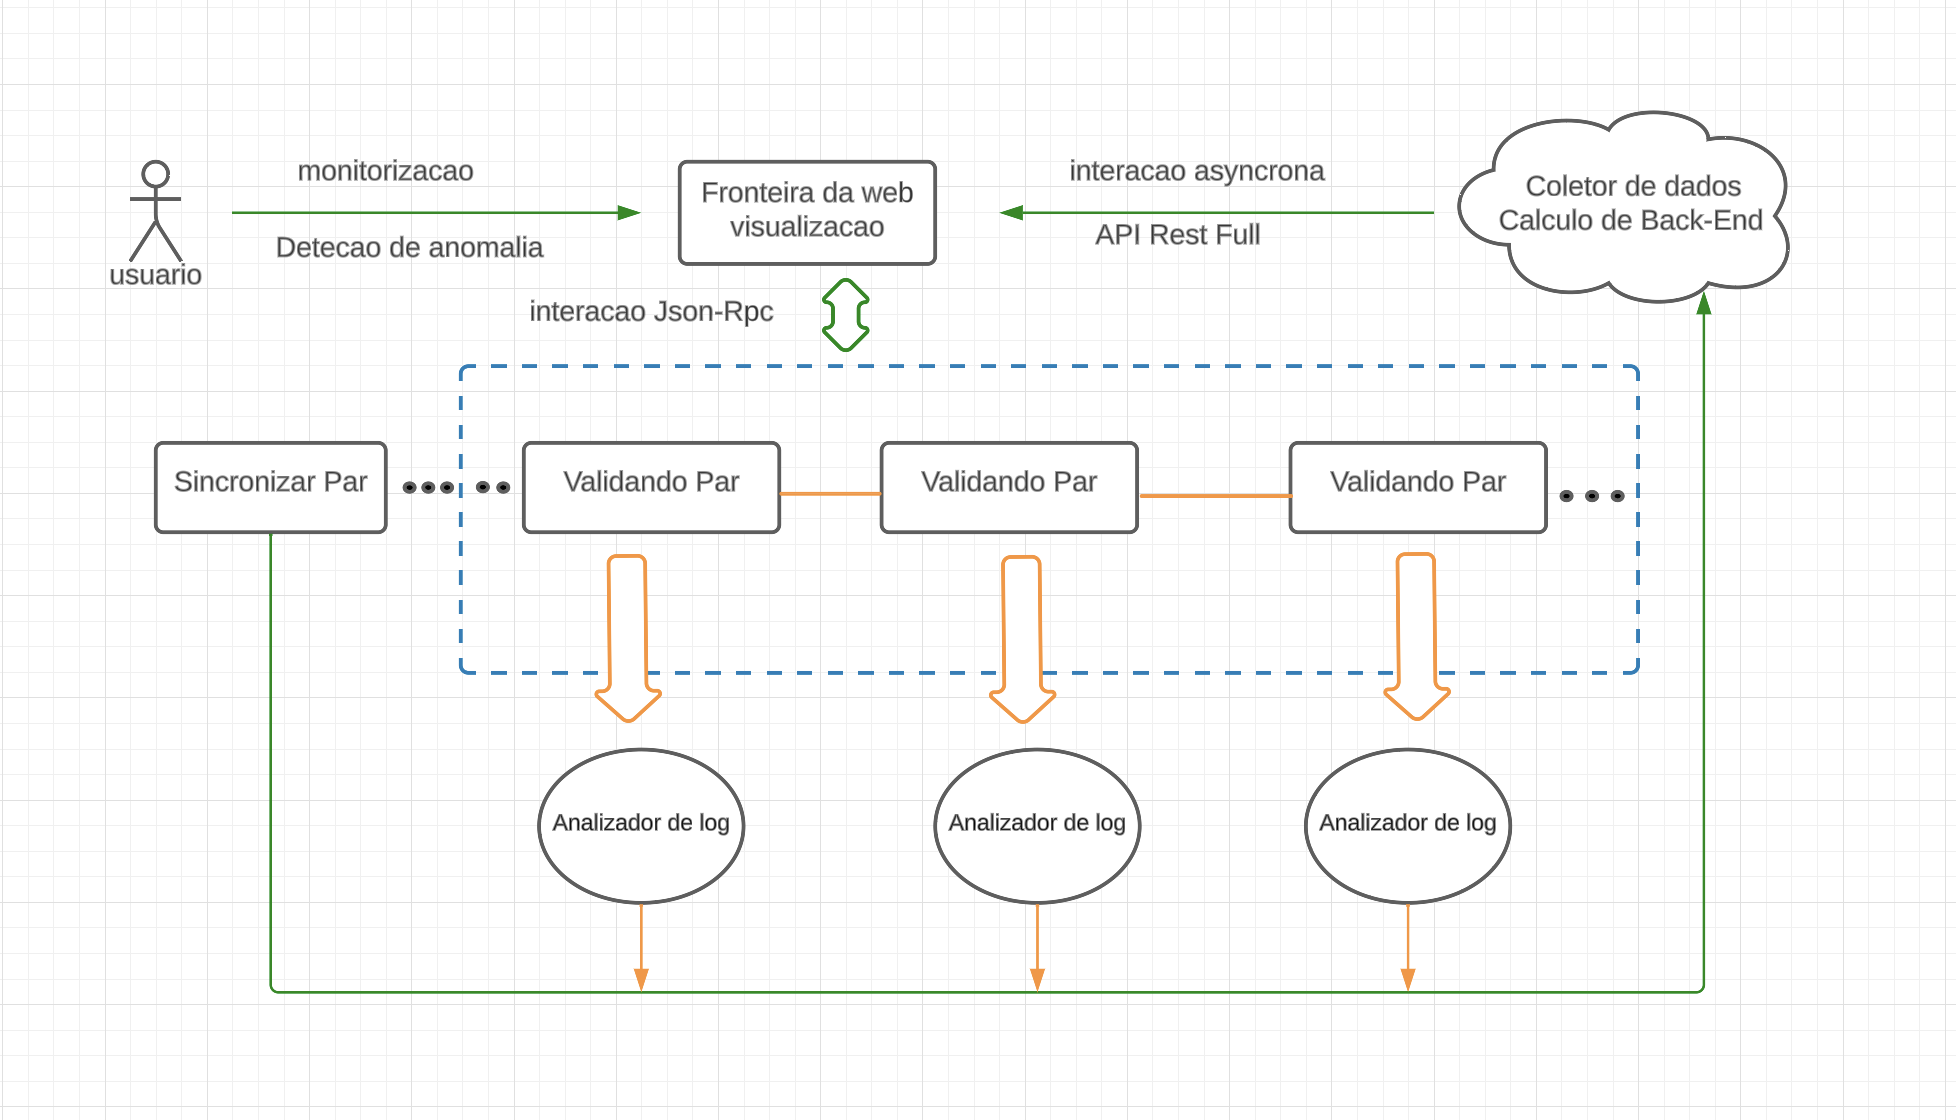
\includegraphics[width=15cm]{4-Analise-de-desempenho-do-Blockchain/figure/monitoramento.png}}
            \caption{Estrutura de monitoramento de desempenho blockchain. \cite{9129732}, .}
            \label{Estrutura de monitoramento}
        \end{figure}
    \subsection{Analise experimental de sistema Blockchain}

    Nesta seção, conduzimos uma análise experimental focada nos sistemas Ethereum, Parity e Hyperledger, com um foco especial na avaliação de seu desempenho. A escolha dessas plataformas foi motivada por sua posição proeminente no domínio do blockchain e pela complexidade e maturidade de seus códigos-base.\cite{comparative-testing}

    \subsubsection{ Etherium }

     Como uma das principais plataformas de contrato inteligente e criptomoedas, Ethereum é amplamente adotado em uma variedade de casos de uso. A  análise de desempenho abrangeu áreas como transações por segundo (TPS), latência, consumo de recursos e escalabilidade. Investiguei como o Ethereum lida com cargas de trabalho crescentes e quais são os principais fatores que afetam seu desempenho.
     %Rouhani e Deter \cite{perfomance-block} estudaram o desempenho do Ethereum para prever a latência de sistema baseados em blockchain privado analisando dois clientes Ethereum mais populares
     
     \subsubsection{ Parity }

     Parity é conhecido por sua eficiência e segurança. Uma breve análise detalhada de seu desempenho, avaliando sua capacidade de processar transações em alta velocidade e como ele se comporta em ambientes de alto volume. Além disso, seu uso em cenários de consórcio e o impacto disso no desempenho.
     
     \subsubsection{Hyperledger}

      Hyperledger é uma plataforma de blockchain empresarial com diversas implementações, incluindo o Hyperledger Fabric e o Hyperledger Sawtooth. A análise se concentrou na comparação de desempenho entre essas implementações, levando em consideração métricas como latência, escalabilidade e eficiência. 
      
     \subsubsection{Análise comparativa}

      Para desenvolver um aplicativo habilitado para Blockchain, os desenvolvedores devem avaliar a adequação da implementação do blockchain. É necessário realizar uma análise comparativa de desempenho para selecionar a plataforma de blockchain que ofereça um desempenho adequado para alcançar os objetivos do aplicativo a ser desenvolvido .

      Após a criação do Blockbench, Dinh et al.\cite{blockbench} empregaram essa ferramenta para conduzir uma análise comparativa de desempenho em três blockchains privados tradicionais: Ethereum (geth v1.4.18), Parity (v1.6.0) e Hyperledger Fabric (HLF v0.6.0-preview). Suas descobertas, baseadas em extensa pesquisa, 

      \begin{itemize}[label= $\star$]
        \item Desempenho Superior do HLF : Notou-se que o Hyperledger Fabric apresenta um desempenho consistentemente superior em relação ao Ethereum e ao Parity em todos os benchmarks, sejam eles de macroescala, como taxa de transferência e latência, ou microescala, como IOHeavy. Isso destaca a robustez do HLF em vários cenários de uso. No entanto, é importante observar que o HLF enfrenta um desafio em termos de escalabilidade, já que não consegue operar eficientemente com mais de 16 nós na rede.

        \item Identificação dos Gargalos: Os autores identificaram que os protocolos de consenso são os principais gargalos para o Hyperledger Fabric e o Ethereum, afetando seu desempenho. Enquanto isso, a assinatura de transações representa um gargalo para o Parity, limitando sua capacidade de processamento.

        Os autores aprofundaram a análise, comparando o desempenho de duas versões distintas do HLF, a v0.6.0 e a v1.0.0, com foco na carga de trabalho IOHeavy. Essa análise adicional proporciona insights valiosos sobre a evolução do desempenho do Hyperledger Fabric ao longo das versões, contribuindo para uma compreensão mais abrangente das capacidades dessas plataformas.\cite{Untangling-blockchain}
      \end{itemize}

      A avaliação de diferentes blockchains continua sendo um desafio devido à ausência de padrões de interface. Como resposta a essa questão, um avanço foi alcançado na forma de uma carga de trabalho genérica que executa as mesmas operações em várias interfaces blockchain. Esse esforço foi notável e pode ser observado em \cite{Evaluating-blockchains}, onde essa carga de trabalho foi concebida. Ela se mostrou essencial para a avaliação comparativa de três proeminentes plataformas de blockchain consórcio para o contexto da Internet das Coisas (IoT). As plataformas em foco incluíram o HLF v0.6 com o consenso Practical Byzantine Fault Tolerance (PBFT), o HLF v1.0 com o consenso de replicação de máquina de estado tolerante a falhas bizantinas (BFT-SMaRt) e o Ripple, que utiliza o consenso Ripple.
      Os resultados dessa avaliação revelaram que os blockchains analisados conseguiram proporcionar uma taxa de transferência razoável. No entanto, destacou-se uma limitação significativa em termos de escalabilidade. Essas descobertas têm implicações cruciais, especialmente em aplicações voltadas para a Internet das Coisas, onde a escalabilidade desempenha um papel vital.
      Esse cenário sublinha a importância contínua de pesquisas e desenvolvimentos em busca de soluções que atendam às crescentes demandas de escalabilidade e eficiência, particularmente em cenários complexos como o da IoT, onde a necessidade de processar grandes volumes de transações de forma confiável é primordial.

      Pongnumkul et al. \cite{Performance-analysis} conduziram uma análise preliminar de desempenho envolvendo duas das plataformas blockchain privadas mais populares: o Hyperledger Fabric (HLF v0.6) e o Ethereum (geth 1.5.8 em implantação privada). Esse estudo avaliou o desempenho sob várias cargas de trabalho, utilizando métricas como tempo de execução, latência e taxa de transferência. Os resultados experimentais demonstraram que o Hyperledger Fabric supera o Ethereum em todas as métricas avaliadas, o que é um indicativo do robusto desempenho do HLF em cenários diversificados.

        No entanto, é importante observar que ambos os sistemas ainda não atingem níveis de desempenho competitivos em comparação com os sistemas de banco de dados tradicionais, especialmente quando submetidos a cargas de trabalho mais elevadas. Essa constatação é reforçada por um estudo mais recente \cite{comparative-testing}, no qual o Ethereum foi comparado com o sistema de gerenciamento de banco de dados MySQL. Os resultados desse estudo corroboraram a conclusão anterior, enfatizando que, embora os blockchains ofereçam vantagens em segurança e descentralização, o desempenho puro ainda precisa ser aprimorado para competir eficazmente com sistemas de banco de dados convencionais.

        A análise comparativa também se estende aos algoritmos de consenso empregados por diferentes blockchains. Por exemplo, Hao et al. \cite{analise-algoritmo-consenso} conduziram uma avaliação comparativa de desempenho entre o Hyperledger (utilizando o algoritmo Practical Byzantine Fault Tolerance - PBFT) e o Ethereum privado (baseado em Proof of Work - PoW). Eles desenvolveram uma estrutura de benchmark abrangente, composta por quatro módulos: um módulo de configuração de carga de trabalho, um módulo de contrato inteligente de consenso, um módulo de coleta de dados e as próprias plataformas blockchain. Os resultados dessa avaliação revelaram que o Hyperledger Fabric supera consistentemente o Ethereum em termos de taxa de transferência média (TPS) e latência. Este estudo destacou a influência significativa do mecanismo de consenso no desempenho de blockchains privados.

        Outro exemplo notável é a análise de desempenho realizada em dois algoritmos de consenso: o Proof of Work (PoW) e a Conjectura Proof-of-Collatz (PCC)\cite{avaliacao-algo-consenso}. O PCC \cite{conjectura} é um algoritmo PoW teórico recentemente introduzido, baseado nas órbitas de Collatz, uma métrica definida no algoritmo da Conjectura de Collatz. Os autores conduziram uma avaliação minuciosa desses algoritmos de consenso, considerando o tempo de execução, o tempo de implantação e a latência em uma rede blockchain privada. Os resultados desses experimentos revelaram que o blockchain baseado na Conjectura Proof-of-Collatz supera consistentemente o blockchain baseado em PoW em todas as métricas avaliadas. Surpreendentemente, alcançou uma velocidade de execução até 1000 vezes mais rápida que o PoW. Esses resultados destacam a importância de inovações em algoritmos de consenso e seu potencial para aprimorar significativamente o desempenho de blockchains.

        % \begin{itemize}[label= $\ast$]
        %     \item \textbf{Analise experimental do desempenho dos três sistemas de blockchain na camada de aplicação}
        % \end{itemize}
        % \textbf{- Execução dos sistemas com benchmarks YCSB e Smallbank em vários nós}

        % \begin{itemize}[label= $\ast$]
        %     \item \textbf{Analise experimental do desempenho do blockchain  com containers Docker}
        % \end{itemize}

    %     \section{Analise experimental do desempenho do blockchain  com containers Docker}
    %     % \textbf{- Estudos de caso}

    %     \subsection{Estudos de caso}

    %     Nesta seção, foi abordado um estudo de caso com o propósito de simular uma rede blockchain por meio da utilização de containers Docker. O principal objetivo dessa simulação foi explorar as potencialidades e desafios associados à implementação de uma infraestrutura baseada em blockchain em um ambiente de contêineres virtualizados. Ao longo do estudo, foram conduzidas diversas atividades para alcançar uma compreensão aprofundada do funcionamento da rede simulada. Inicialmente, foram configurados e interligados os containers Docker, replicando assim a estrutura distribuída de uma rede blockchain. Esta fase envolveu a criação de nós, a definição de suas interações e a configuração de parâmetros específicos.

    %     Optei por concentrar a pesquisa no registro de diplomas digitais, apesar das diversas aplicações potenciais para a simulação de Blockchain. Essa decisão estratégica foi motivada pela complexidade e relevância específicas desse cenário, destacando-se, em parte, devido às limitações observadas ao tentar utilizar outros simuladores. Muitas vezes, essas plataformas carecem dos recursos tecnológicos necessários para realizar testes abrangentes e coletar resultados de maneira eficaz.

    %     Morais (2019) sugere que instituições de ensino possuam a capacidade de emitir diplomas e certificados em formato digital, com a proposta de registrar esses documentos em uma Blockchain para garantir sua autenticidade. Esse conceito envolve a geração de um identificador único para cada documento, que, uma vez registrado na Blockchain, estabelece uma referência permanente. Isso viabiliza a verificação da existência do documento original sempre que necessário.

        
    %     % Acredito que essa abordagem proporcionará uma compreensão mais aprofundada das implicações práticas da implementação do Blockchain no registro de documentos educacionais digitais, aproveitando ao máximo as vantagens tecnológicas e superando obstáculos anteriores.

    %     Ao selecionar o registro de diplomas digitais como foco da pesquisa, não apenas busco explorar a eficácia do Blockchain nesse contexto específico, mas também superar as limitações encontradas em outros simuladores.A simulação, desenvolvida em Node.js, cria o bloco gênesis da cadeia e estabelece os nós da Blockchain em containers por meio do Docker. Cada container é equipado com uma imagem Linux que armazena uma réplica dos registros da cadeia de blocos. Após a inicialização, os nós passam a monitorar a validade dos novos blocos adicionados, decidindo se podem ser integrados à rede.
    %     Neste estudo, a quantidade de nós a ser instanciada é determinada pelo pesquisador. Inicialmente, optei por simular uma rede com 10 nós, representando um ambiente de pequena escala. Posteriormente, esse número foi aumentado para 20, com o objetivo de observar o comportamento da rede com o dobro de nós. Ao ser executada, a aplicação gera exclusivamente o bloco gênesis, marcando o início da cadeia, e o distribui para todos os nós. A partir desse ponto, os nós monitoram a validade dos novos blocos adicionados, decidindo se eles podem ser integrados à cadeia.

    %     Os testes foram realizados em um sistema operacional Linux Mint 19.1 de 64 bits. A Figura \ref{Bloco 0} exibe uma representação visual da rede Blockchain gerada pela aplicação, destacando o bloco gênesis da cadeia, o timestamp que indica o momento de sua geração, e o hash de identificação correspondente.

    %     \begin{figure}[H]
    %         \centering
    %         \frame{\includegraphics[width=15cm]{4-Analise-de-desempenho-do-Blockchain/figure/Capture d’écran 2023-12-03 à 18.35.20.png}}
    %         \caption{Representação grafica do primeiro bloco .}
    %         \label{Bloco 0}
    %     \end{figure}


        
        

    % %     YCSB (Yahoo Cloud Serving Benchmark): O YCSB é uma ferramenta de benchmark amplamente utilizada para avaliar o desempenho de sistemas de armazenamento e bancos de dados, incluindo sistemas de banco de dados NoSQL. Ele permite medir a capacidade de um sistema de processar cargas de trabalho de leitura e gravação de dados em uma ampla gama de cenários. Isso ajuda a determinar como um sistema se comporta sob diferentes condições de uso, como o número de operações por segundo, latência e escalabilidade.
        
    % %     Smallbank: Smallbank é outro benchmark projetado para medir o desempenho de sistemas de gerenciamento de bancos de dados em cenários de processamento de transações. Ele simula um conjunto de operações bancárias comuns, como saques, depósitos e transferências, e avalia como um sistema lida com essas transações em termos de taxa de transferência, latência e eficiência.

    % %     \begin{itemize}[label= $\blacklozenge$]
    % %         \item \textbf{Throughput and latency(Taxa de transferência e latência):} 
    % %         Foi avaliado o desempenho máximo dos três sistemas usando 8 servidores e 8 clientes simultâneos durante um período de 5 minutos. Cada cliente enviou transações para um servidor com uma taxa variando de 8 tx/s a 1024 tx/s. Os resultados demonstram que o Hyperledger supera outros sistemas em termos de taxa de transferência, com um desempenho até 5,5 vezes maior que o Ethereum e 28 vezes maior que o Parity. Figure \ref{Blockchain performance}

    % %         A diferença entre o desempenho do Hyperledger e Ethereum se deve ao protocolo de consenso, sendo o primeiro baseado no PBFT (Practical Byzantine Fault Tolerance) e o segundo no PoW (Proof of Work). Com 8 servidores, o custo de comunicação na transmissão de mensagens no Hyperledger é significativamente mais eficiente do que a mineração de blocos, que possui uma dificuldade ajustada para cerca de 2,5 segundos por bloco.Figure \ref{Blockchain performance}.b
    % % \begin{figure}[H]
    % %         \centering
    % %         \frame{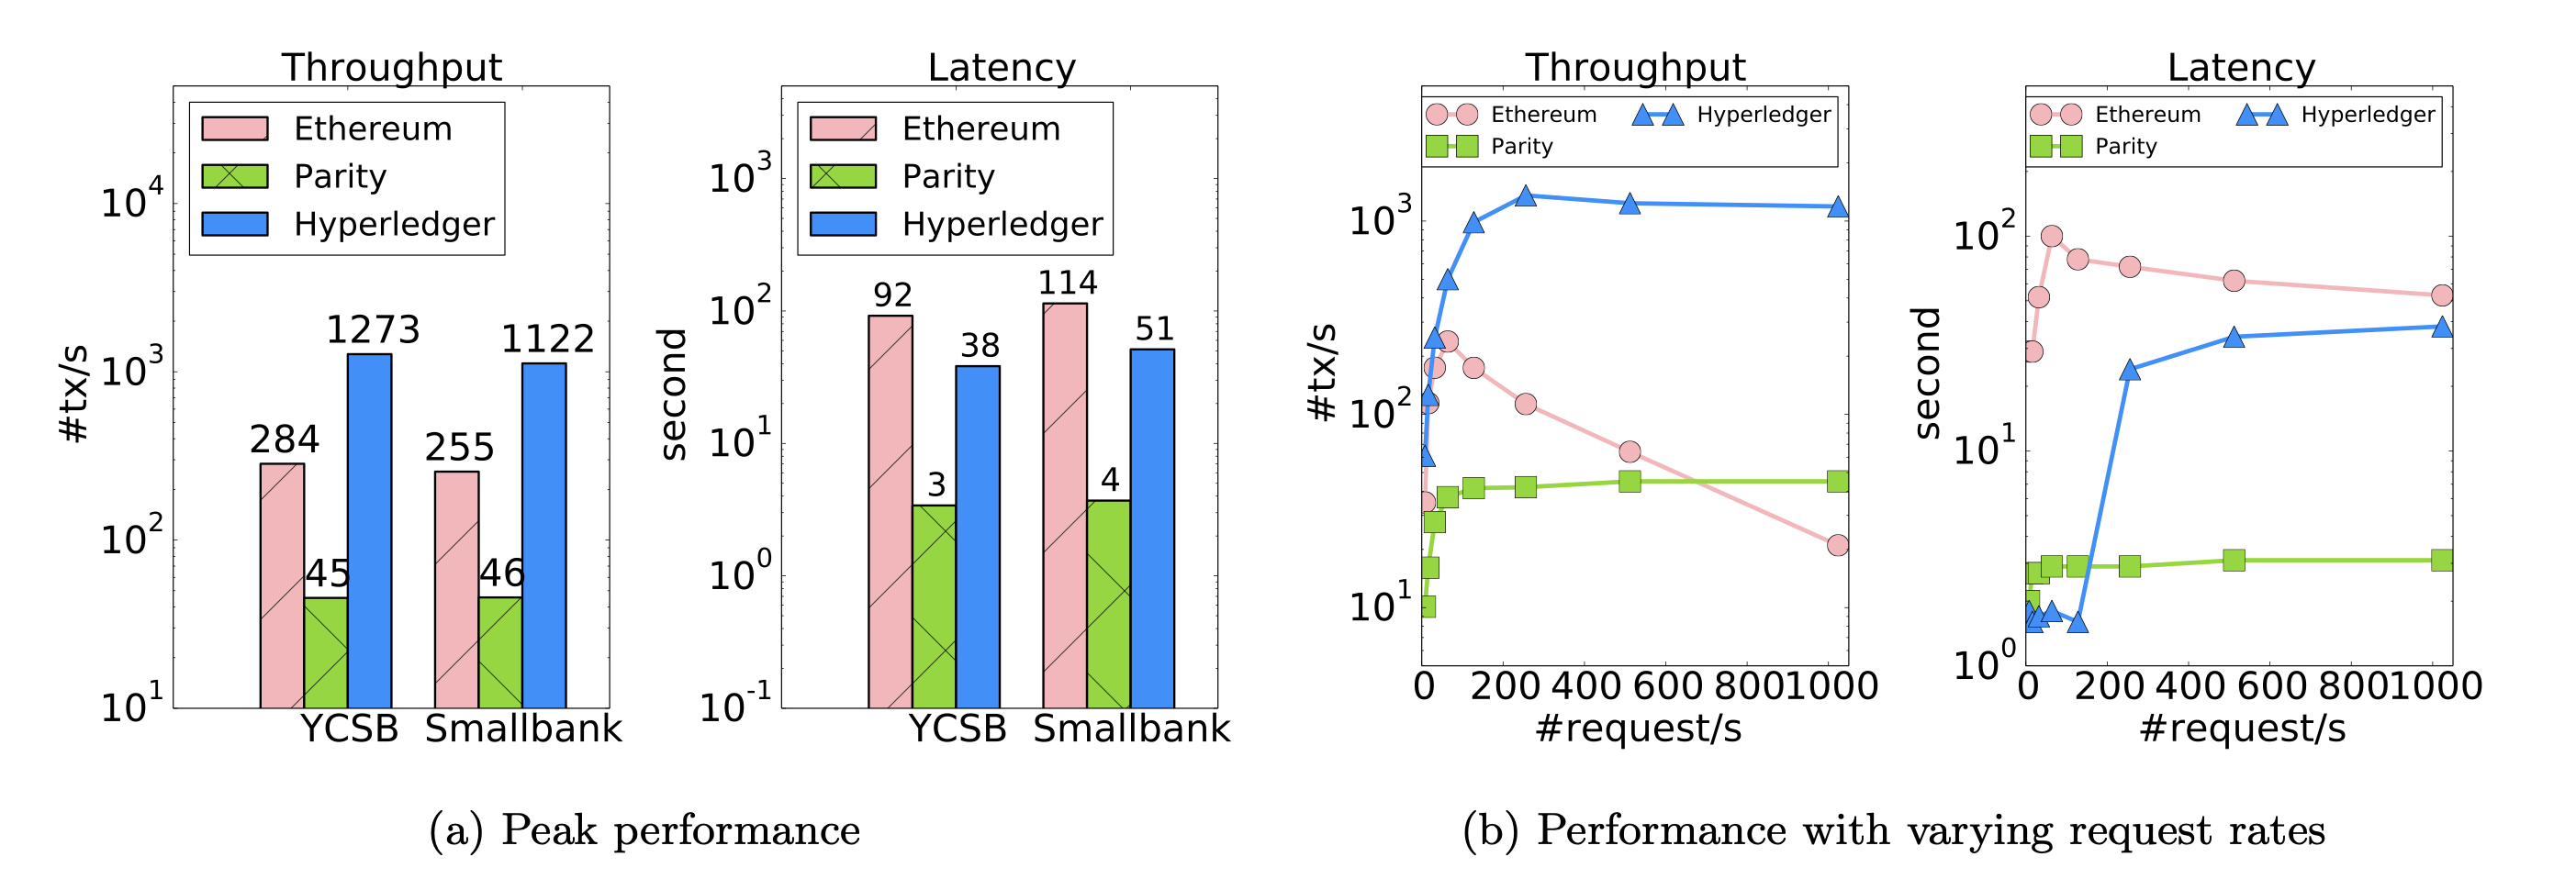
\includegraphics[width=15cm]{4-Analise-de-desempenho-do-Blockchain/figure/Blockchain-perfomance.png}}
    % %         \caption{Blockchain performance with 8 clients and 8 servers. \cite{blockbench}, .}
    % %         \label{Blockchain performance}
    % %     \end{figure}

    % %         A Figura \ref{clients request} compara os tamanhos da fila antes e depois de os sistemas atingirem seu pico de taxa de transferência. Com apenas 8 tx/s, as filas do Ethereum e Hyperledger permanecem em tamanhos aproximadamente constantes, mas o tamanho da fila do Parity aumenta com o tempo. Mais interessante ainda, sob cargas elevadas (512 tx/s por cliente), a fila do Parity é sempre menor do que a do Ethereum e do Hyperledger.
    % %         O desempenho do Parity, por sua vez, não é afetado pelo protocolo de consenso, visto que o PoA (Proof of Authority) é esperado como mais eficiente. O Parity mantém uma taxa de transferência e latência constantes, mesmo sob cargas elevadas. Isso sugere que o Parity processa transações a uma taxa constante e impõe um limite máximo na taxa de solicitação de clientes, obtendo, assim, uma menor taxa de transferência e latência em comparação com outros sistemas.

    % %         \begin{figure}[H]
    % %             \centering
    % %             \frame{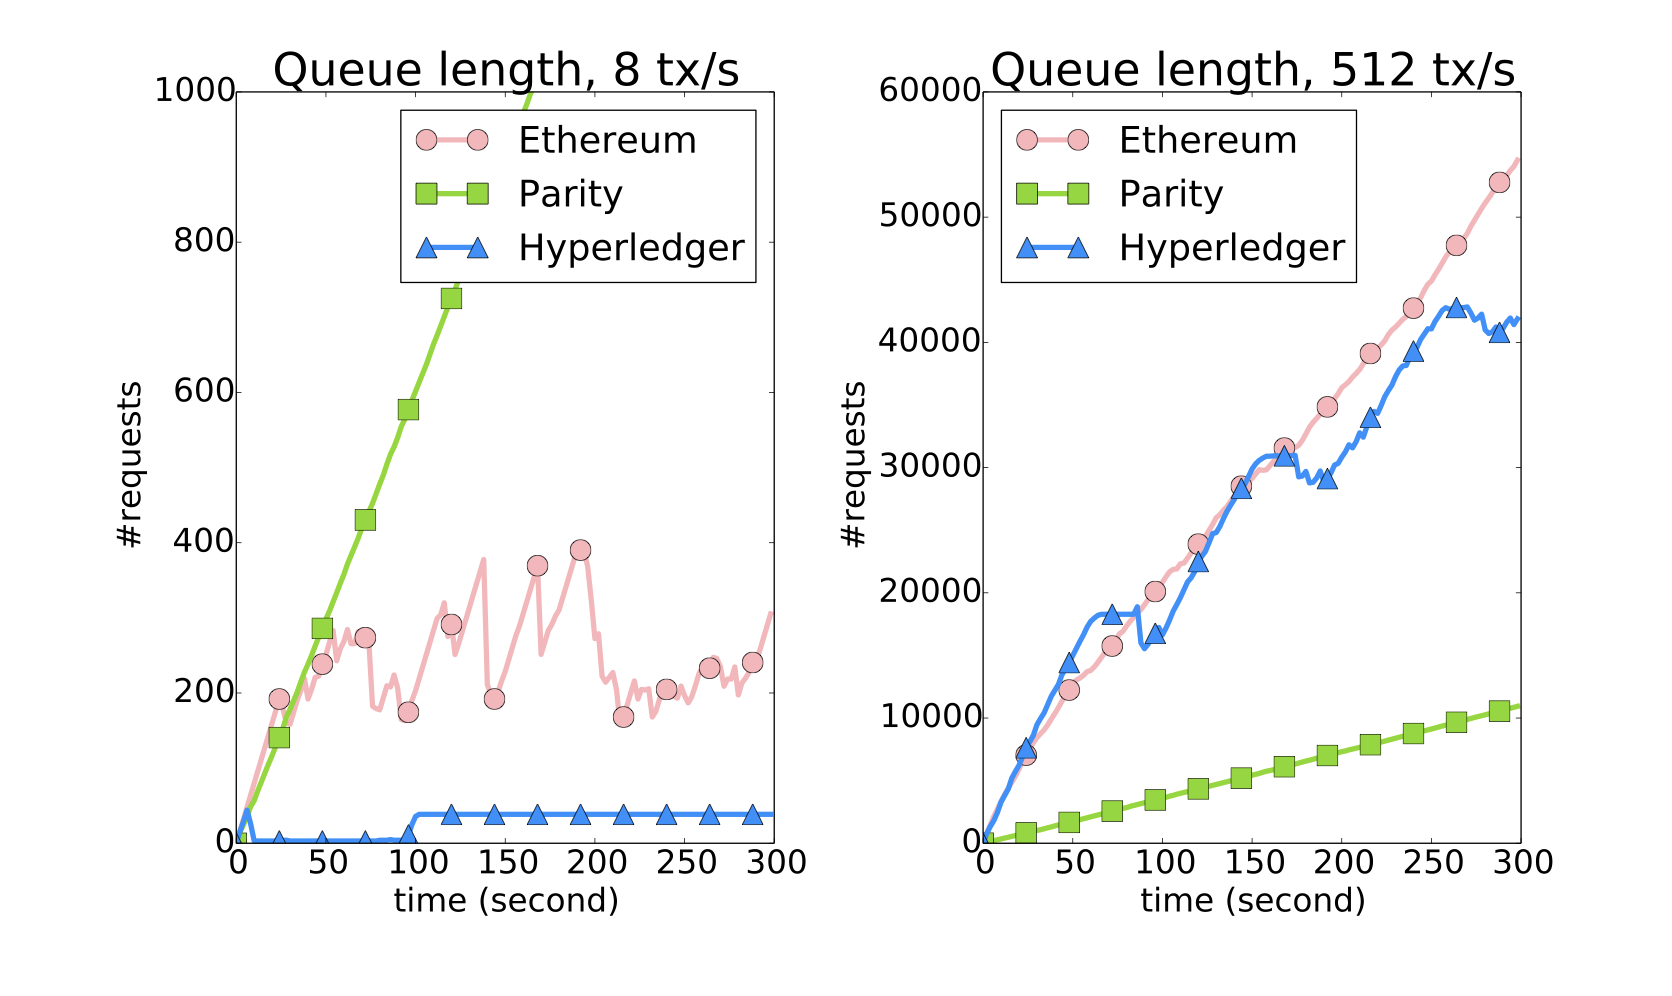
\includegraphics[width=15cm]{4-Analise-de-desempenho-do-Blockchain/figure/Clients request.png}}
    % %             \caption{Client’s request queue, for request rates of 8 tx/s and 512 tx/s \cite{blockbench}, .}
    % %             \label{clients request}
    % %         \end{figure}

    % %         Além disso, foram observadas diferenças nas cargas de trabalho YCSB e Smallbank, resultando em uma redução de 10\% na taxa de transferência e um aumento de 20\% na latência. Isso ocorre porque a execução de contratos inteligentes Smallbank é mais onerosa, envolvendo mais leituras e gravações nos estados do blockchain.

    % %         No pico de sua taxa de transferência, o Hyperledger gera 3,1 blocos por segundo e atinge uma taxa de transferência total de 1273 tx/s, embora ainda seja menor do que a de sistemas de banco de dados em memória. Os resultados também demonstram que, com o aumento do tamanho dos blocos, a taxa de geração de blocos diminui proporcionalmente, sem melhoria na taxa de transferência global.
    % %     \end{itemize}
        

       
